% $Id: board1.tex 10137 2022-06-04 20:51:54Z mskala $

%
% MSK 013 Board 1 build instructions
% Copyright (C) 2020  Matthew Skala
%
% This program is free software: you can redistribute it and/or modify
% it under the terms of the GNU General Public License as published by
% the Free Software Foundation, version 3.
%
% This program is distributed in the hope that it will be useful,
% but WITHOUT ANY WARRANTY; without even the implied warranty of
% MERCHANTABILITY or FITNESS FOR A PARTICULAR PURPOSE.  See the
% GNU General Public License for more details.
%
% You should have received a copy of the GNU General Public License
% along with this program.  If not, see <http://www.gnu.org/licenses/>.
%
% Matthew Skala
% https://northcoastsynthesis.com/
% mskala@northcoastsynthesis.com
%

\chapter{Building Board 1}\label{ch:board1}

Board~1 has components on both sides, and for best results, it is important
to install them in the right order.  Build Board~2 first, and see the
general comments in the Board~2 chapters about how to approach the task.

\section{Preliminaries}

Count out the right number of everything according to the bill of materials. 
There is an abbreviated BOM for the items needed in this chapter (including
the connection to Board~2 and final assembly of the module) in
Table~\ref{tab:b1bom}.

\nopagebreak
\noindent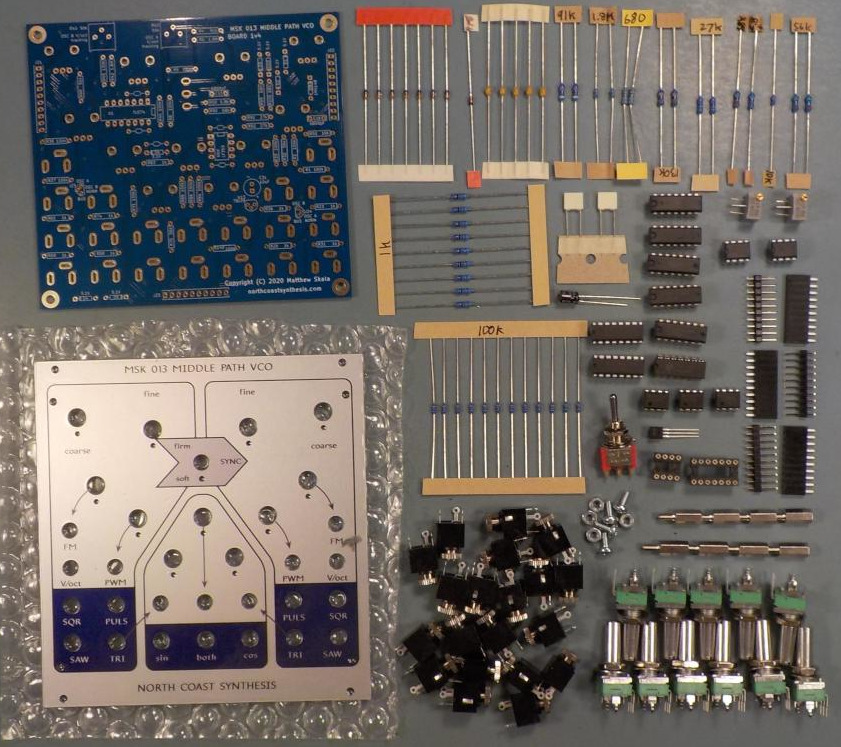
\includegraphics[width=\linewidth]{board1-parts.jpg}

\begin{table*}
{\centering
\fbox{This table is not a substitute for the text instructions.}
\vspace{\baselineskip}

\begin{tabular}{rp{1.4in}cp{2.9in}}
  \textbf{Qty} & \textbf{Ref} & \textbf{Value/Part No.} & \\ \hline
\input{bomdata-1.tex}
\end{tabular}\par}
\caption{Bill of Materials for Board~1 and the final assembly of
the module.  Also needed:
the PCB itself, the aluminum front panel, knobs, the assembled Board~2, and
panel-to-rack mounting hardware.  Note some kits may substitute parts of
equivalent or better specifications, in particular 1N5231C Zener diodes and
TL074B op amps.}\label{tab:b1bom}

\end{table*}

\section{Some notes on knobs}

The first batch of knobs I ordered for North Coast products turned out to
have serious quality problems, specifically with the setscrews that hold the
knobs onto the potentiometer shafts.  Some of the screws had marginal
threads that would strip when the screw was tightened, and I ended up having
to do a bunch of extra testing and ship extra knobs to some customers to
replace any that might fail.  Later batches have also had issues, although
they're under better control now because the bad first batch served as a
warning to step up the testing procedures.

Starting with kits prepared in August 2019 (including all Middle Path VCO
kits), I switched to blue knobs with 100\%\ testing; in September 2020, I
switched to a new manufacturer, and knobs that are a slightly darker shade
of blue.  Although all the knobs I ship in kits now have been tested and
passed at least twice, and should be fine to use, I am also shipping spare
setscrews in any kits with knobs from batches where a signficant number of
knobs failed testing.

\section{Normalization selection}

In a standard build, the V/oct input of the master oscillator is normalized
to the Eurorack bus CV, and that of the slave oscillator is normalized to
the V/oct input of the master oscillator.  As a result, the control scheme
for the two oscillators works as follows.
\begin{itemize}
  \item With no cables plugged into the V/oct jack sockets:  both
    oscillators controlled by bus CV.
  \item With a cable plugged into the master V/oct jack socket only:  both
    oscillators controlled by the cable CV.
  \item With a cable plugged into the slave V/oct jack socket only:  master
    controlled by bus CV, slave by the cable CV.
  \item With cables pluegged into both V/oct jack sockets:  each oscillator
    controlled by its own cable.
\end{itemize}

However, if desired you can change these normalizations by cutting and
bridging some traces on the Board~1 PCB.  For example, if you don't want to
use the CV bus, or do want to use it for some other purpose, you could
remove the connection to that.  In all cases, if a cable is plugged into an
oscillator's own V/oct jack socket then the oscillator will use that cable's
CV in preference to any other source of V/oct control; the normalization
only controls what happens if there is no cable, with options of bus CV, the
other oscillator's CV (which could have also come from a normalization), or
nothing.  Normalizing both oscillators across to each other means they both
get the equivalent of 0V when no cables are plugged in, and a single cable
plugged into either will control both.

There are two jumper footprints, shown on the schematic as SPDT switch
symbols J24 and J25, for oscillator A (master) and oscillator B (slave)
respectively.  Each consists of three pads, with the centre pad joined to
one of the side pads for the default normalization.  Cut that connection to
have no normalization (equivalent to being normalized to 0V); cut it and
also join the middle pad to the pad on the other side with a bit of wire or
a blob of solder, to normalize to the other option.  As marked on the board,
oscillator A can normalize to ``BUS'' (default) or ``OSC~B,'' and oscillator
B can normalize to ``BUS'' or ``OSC~A'' (default).

\noindent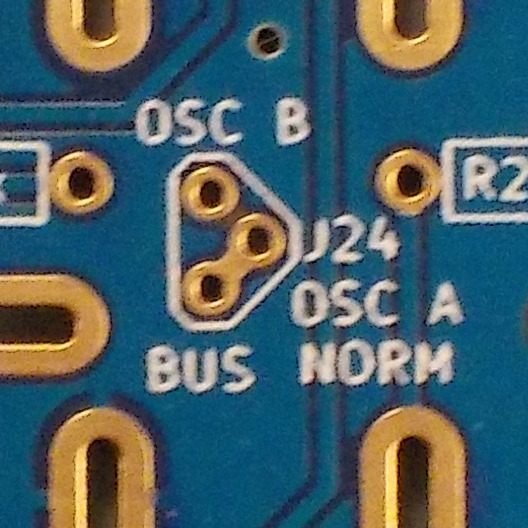
\includegraphics[width={1.50in}]{osca-norm.jpg}\quad
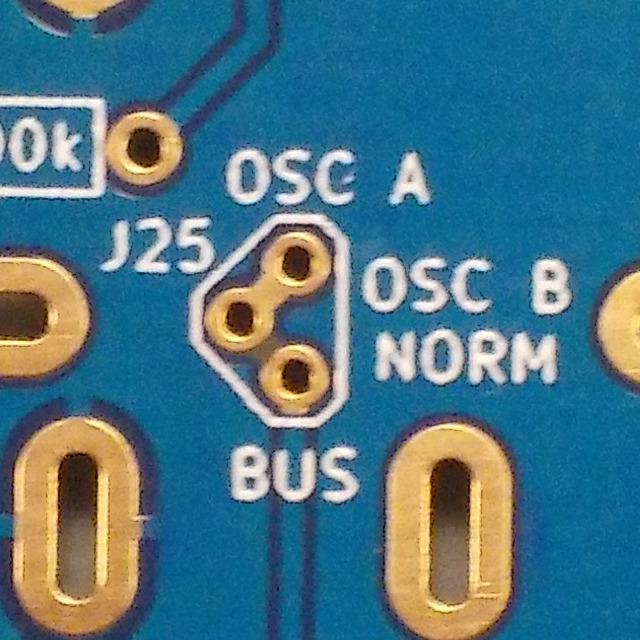
\includegraphics[width={1.50in}]{oscb-norm.jpg}

If you want to do this modification then do it now, before installing
components on the board.  Use an ohmmeter across the pads to check that the
connection you intended to break really is broken, and that any connection
you intended to add really has become connected.

If you sell a modified build, please tell the buyer that it is modified.

\section{Decoupling capacitors}

The five axial ceramic 0.1$\mu$F decoupling capacitors C28, C28, and
C32--C34 are shown on
the board by a special symbol without their reference designators.

\nopagebreak
\noindent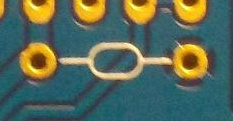
\includegraphics[width=\linewidth]{decoup-symbol.jpg}

\pagebreak

Install these capacitors where the symbol appears.  They are not
polarized and may be installed in either orientation.  These capacitors act
as filters for the power supplies.

\nopagebreak
\noindent\includegraphics[width=\linewidth]{{cap-0.1u1}.jpg}

\section{Fixed resistors}

Resistors are never polarized.  I like to install mine in a consistent
direction for cosmetic reasons, but this is electrically unnecessary.  In
this module, the fixed resistors are metal film 1\%\ type.  They usually
have blue bodies and four colour bands designating the value, plus a fifth
band for the tolerance.  The tolerance band is brown for 1\%, but note that
we may occasionally ship better-tolerance resistors in the kits than the
specifications require, if we are able to source them at a good price. 
Accordingly, I mention only the four value band colours for this type of
resistor; if you are using resistors with other codes, you are responsible
for knowing them.  Note that colour codes on metal film 1\% resistors are
often ambiguous (reading from one end or the other end may give two
different values, both plausible) and some of the colours are hard to
distinguish anyway.  If in doubt, always measure with an ohmmeter before
soldering the resistor in place.

\pagebreak

Install the two 680$\Omega$ (blue-grey-black-black) resistors R93 and R105.
These are the first and last of the resistors in the chain that drives the
transistor basis in the sine shaper; the others were already installed on
Board~2.  Do not confuse them with the 6.8k$\Omega$ and 68k$\Omega$
resistors.

\nopagebreak
\noindent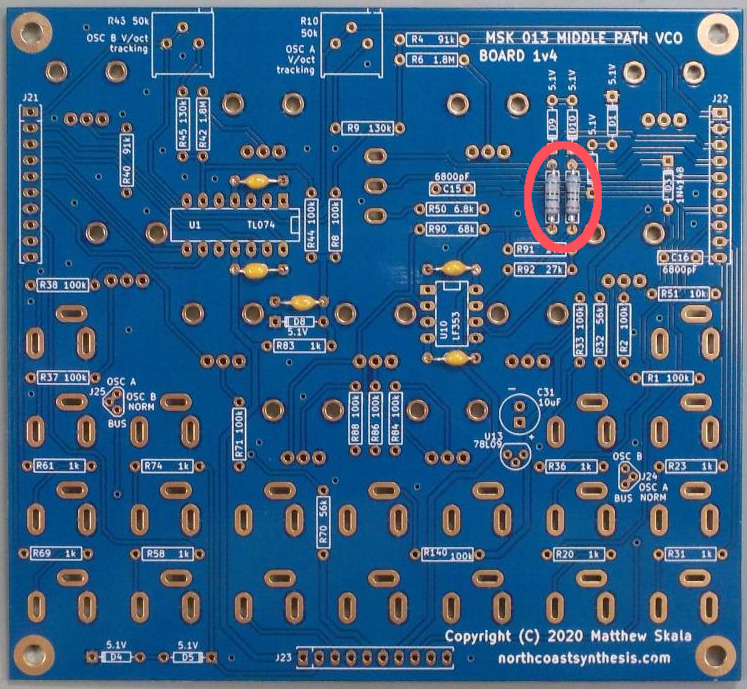
\includegraphics[width=\linewidth]{res-680-1.jpg}

Install the nine 1k$\Omega$ (brown-black-black-brown) resistors R20, R23,
R31, R36, R58, R61, R69, R74, and R83.  Most of these are for limiting
current and ensuring stability on op amps that drive output jacks.  R83 is a
ballast resistor for the $-$5V reference supply regulator.  Do not confuse
these with other power-of-ten values, such as 10k$\Omega$ and 100k$\Omega$.

\nopagebreak
\noindent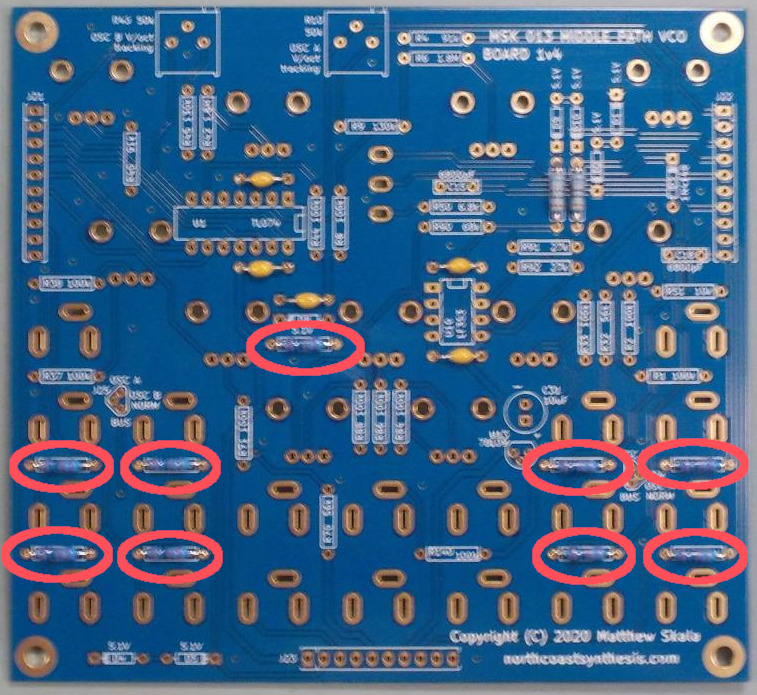
\includegraphics[width=\linewidth]{res-1k1.jpg}

\pagebreak

Install the single 6.8k$\Omega$ (blue-grey-black-brown) resistor R50.  This
resistor couples sync pulses from the master to the slave oscillator in
``firm'' sync mode.  Do not confuse it with the 68k$\Omega$ resistor.

\nopagebreak
\noindent\includegraphics[width=\linewidth]{{res-6.8k1}.jpg}

Install the single 10k$\Omega$ (brown-black-black-red) resistor R51. 
This resistor provides recharging current for the capacitor in the soft sync
circuit.

\nopagebreak
\noindent\includegraphics[width=\linewidth]{{res-10k1}.jpg}

\pagebreak

Install the two 27k$\Omega$ (red-violet-black-red) resistors R91 and R92. 
These set gain for an inverting amplifier in the sine shaper.

\nopagebreak
\noindent\includegraphics[width=\linewidth]{{res-27k1}.jpg}

Install the two 56k$\Omega$ (green-blue-black-red) resistors R32 and R70. 
These set the normalling voltage for the PWM inputs.

\nopagebreak
\noindent\includegraphics[width=\linewidth]{{res-56k}.jpg}

\pagebreak

Install the single 68k$\Omega$ (blue-grey-black-red) resistor R90.  This
resistor sets the gain for the mixing amplifier in the sine shaper.  It is
the last resistor in the build with a ``68'' code, but double check that
this resistor really is 68k$\Omega$ and not the similarly-coded 680$\Omega$
or 6.8k$\Omega$ value.

\nopagebreak
\noindent\includegraphics[width=\linewidth]{{res-68k}.jpg}

Install the two 91k$\Omega$ (white-brown-black-red) resistors R4 and R40. 
These set the scale factor for the coarse tuning knobs.

\nopagebreak
\noindent\includegraphics[width=\linewidth]{{res-91k}.jpg}

\pagebreak

Install the twelve 100k$\Omega$ (brown-black-black-orange) resistors
R1, R2, R8, R33, R37, R38, R44, R71, R84, R86, R88, and R140.  Most of these
are used to set input impedances in op amps that take input from the outside
world.  R4 and R44 set the offset for the exponential converters,
effectively the frequency at 0V control input; and R140 sets the normalling
voltage for the sine shaper's middle input.  These are the last power-of-ten
fixed resistors in the build sequence.

\nopagebreak
\noindent\includegraphics[width=\linewidth]{{res-100k1}.jpg}

Install the two 130k$\Omega$ (brown-orange-black-orange) resistors R4 and
R45.  These resistors, along with the trimmers to be installed later, set
the gain for the input amplifiers in the exponential converter.

\nopagebreak
\noindent\includegraphics[width=\linewidth]{{res-130k}.jpg}

\pagebreak

Install the two 1.8M$\Omega$ resistors (brown-grey-black-yellow) resistors
R6 and R42.  These set the scale factor for the fine tuning knobs.  It is
possible that some kits may ship with resistors coded 1.82M$\Omega$
(brown-grey-red-yellow) instead of 1.80M$\Omega$.  Either is close enough.

\nopagebreak
\noindent\includegraphics[width=\linewidth]{{res-1.8m}.jpg}

\section{Semiconductors}

There are two different kinds of diodes to install on this board and they
look almost exactly alike: one 1N4148 or 1N914 switching diode named D3, and
seven 1N5231B or equivalent 5.1V Zener diodes named D1, D2, D4, D5, and
D8--D10.  All three
diodes will be packaged in little pink glass beads with near-microscopic
etched numbers indicating their type.  Be careful not to confuse them;
swapping the switching diode with a Zener will result in incorrect behaviour
of the full-wave rectifier at high input voltages, and incorrect feedback
levels probably causing either very strong oscillation at all resonance
settings, or preventing oscillation entirely.

If you are unsure which diode is which and you cannot confidently read the
etched markings, hook up a diode in series with a 10k$\Omega$ resistor
reverse-biased across a 12V power supply and measure the voltage drop across
the diode.  If it is near 12V, then you are testing the switching diode; if
it is near 5.1V, you are testing one of the Zener diodes; if it is near
0.6V, you probably have the diode connected forward-biased and should
reverse it or the power supply.

Both kinds of diodes are polarized and must be installed in the correct
direction to function properly.  One end of the glass body of the diode
package will be labelled with a black band or stripe; that end is the
\emph{cathode}.  The direction for the cathode is marked on the PCB
silkscreen by a matching stripe in the printed symbol; and the solder pad
for the cathode is square rather than round.  There are also labels saying
``5.1V'' and ``1N4148'' next to the diode footprints as additional clues to
which diode goes where.

Install the switching diode D3, bearing in mind the notes above.  This diode
separates the rising and falling edges in soft sync mode.

\nopagebreak
\noindent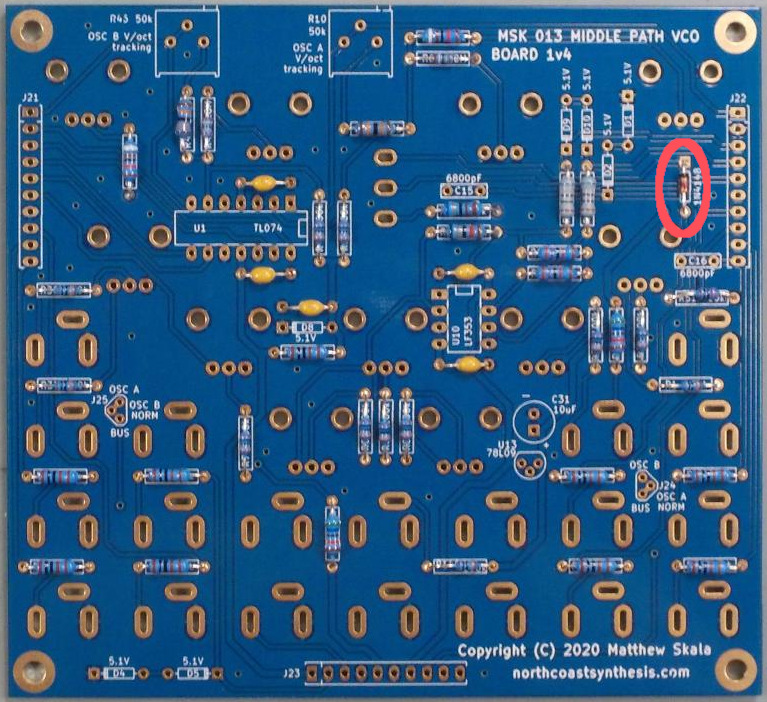
\includegraphics[width=\linewidth]{1n4148.jpg}

Install the seven 5.1V Zener diodes D1, D2, D4, D5, and D8--D10.  Most of
these are used in pairs to clip signal voltages, in the pulse and sine
shapers.  D8 is used to regulate a negative voltage offset for the
exponential converter.

\nopagebreak
\noindent\includegraphics[width=\linewidth]{{zener-5.1v}.jpg}

Install the 8-pin DIP socket for the LF353 dual operational amplifier U10. 
The amplifiers in this chip drive the two ends of the resistor chain for the
sine shaper.

\nopagebreak
\noindent\includegraphics[width=\linewidth]{{dip8-1}.jpg}

Recall from the Board~2 build that DIP sockets themselves do not care which
direction you install them, but it is critically important that the chip
installed in the socket should be installed in the right direction.  To help
with that, the socket will probably be marked with notches at one end
(indicating the end where Pin~1 and Pin~8, or Pin~14 as applicable, are
located) and you should install the socket so that the notched end matches
the notch shown on the PCB silkscreen.  The solder pad for Pin~1 is also
distinguished by being rectangular instead of rounded.

Installing DIP sockets without having them tilted at a funny angle can be
tricky.  I recommend inserting the socket in the board, taping it in place
on the component side with vinyl electrical tape or sticking it there with a
small blob of putty at each end, then soldering one pin on
one corner and checking that the socket is snug against the board before
soldering the other pins.  That way, if you accidentally solder the first
pin with the socket tilted, it will be easier to correct (only one pin to
desolder instead of all of them).

\pagebreak

Install the 14-pin DIP socket for the TL074 quad operational amplifier U1. 
The amplifiers in this chip process pitch control voltages and drive the
reference current sources for the dual exponential converter.

\nopagebreak
\noindent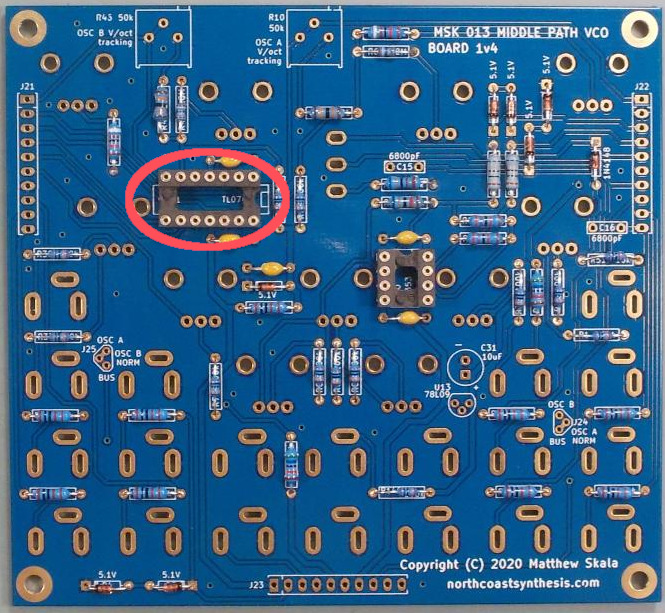
\includegraphics[width=\linewidth]{dip14-1.jpg}

Install the 78L09 regulator U13.  See page~\pageref{pag:to-92} in the
Board~2 instructions for general comments on how to install TO-92 components
like this one.  This regulator provides a +9V reference used in the
exponential converter.

\nopagebreak
\noindent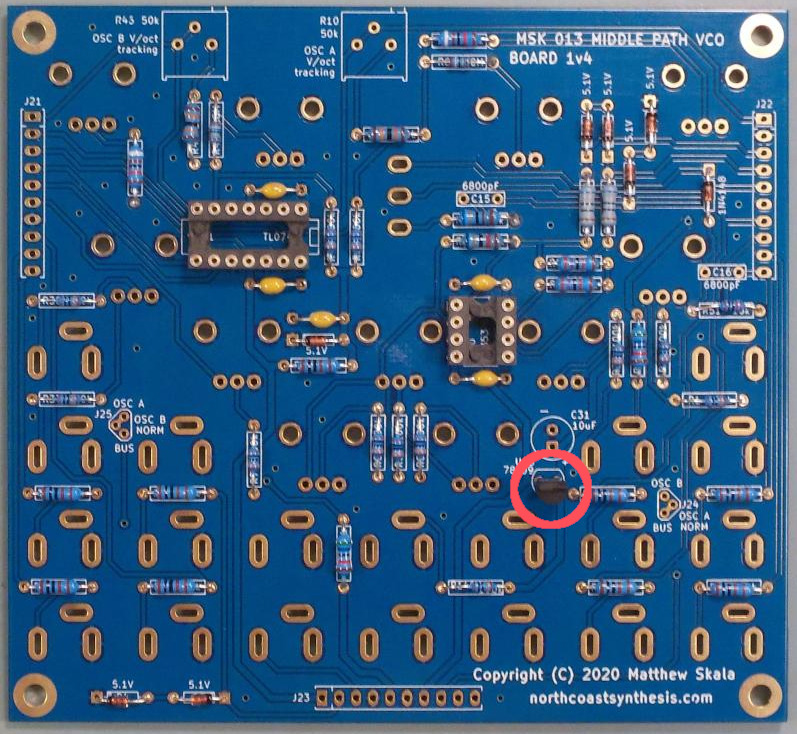
\includegraphics[width=\linewidth]{78l09.jpg}

\pagebreak

\section{Trimmer potentiometers}

Trimmers are not exactly polarized, but the three legs of each trimmer serve
different functions and need to be connected to the right holes.  The
physical arrangement of the legs and corresponding holes should make it
impossible to install the trimmers wrong way round.

Install the two 50k$\Omega$ multiturn trimmers R10 and R46.  These trimmers
set the scale factor for the V/octave pitch CVs of the two oscillators, an
adjustment often called ``tracking.''

\nopagebreak
\noindent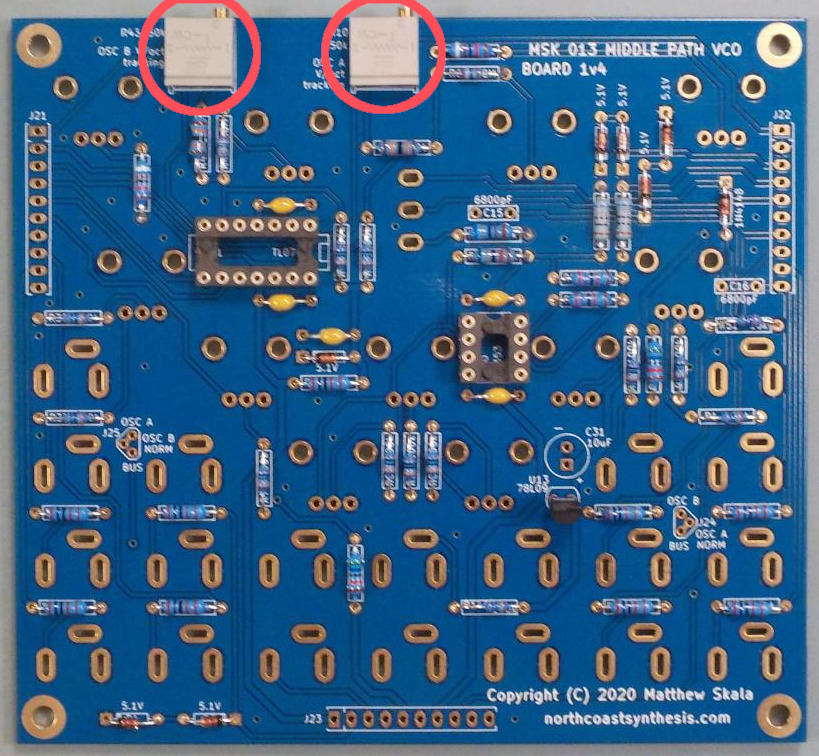
\includegraphics[width=\linewidth]{trim-50k.jpg}

\section{More capacitors}

Install the two 6800pF film capacitors C15 and C16.  These are coupling
capacitors used in the sync circuit.  They are unpolarized and may be
installed in either direction.  The markings on film capacitors vary
depending on the manufacturer and model.  These ones might be marked ``682''
(for 68 followed by two 0s number of picofarads, like the resistor code),
``6n8'' (for 6.8nF), or even ``0.0068'' (value in $\mu$F).

\nopagebreak
\noindent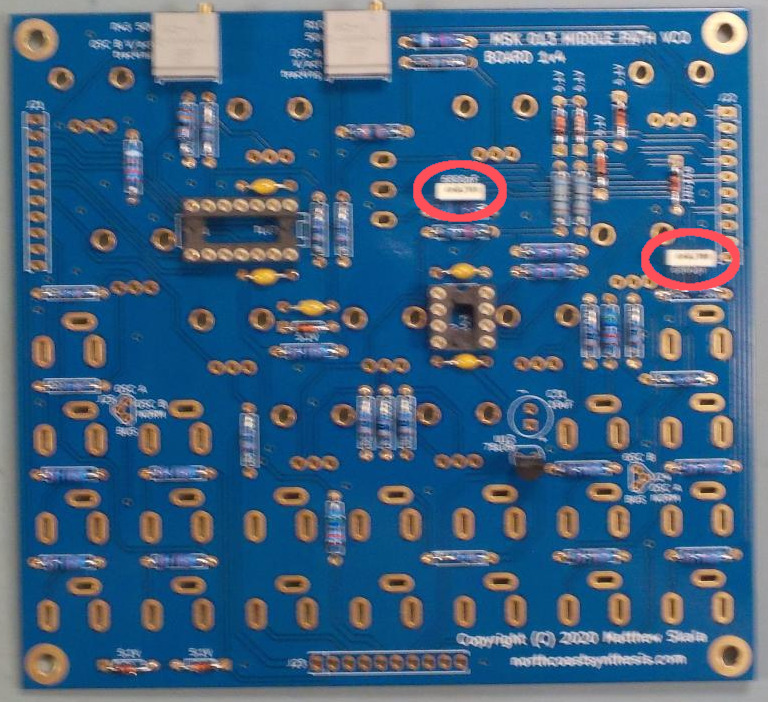
\includegraphics[width=\linewidth]{cap-6800p.jpg}

Install the 10$\mu$F electrolytic capacitor C31.  This filters the +9V
reference voltage.  It is a polarized component and may explode if installed
backwards.  It will be marked on its casing with a stripe and minus
signs to indicate the negative lead; the positive lead will probably also be
longer.  These clues should be matched with the markings on the PCB: plus
and minus symbols in the silkscreen and a square solder pad for the positive
(long) lead.

\nopagebreak
\noindent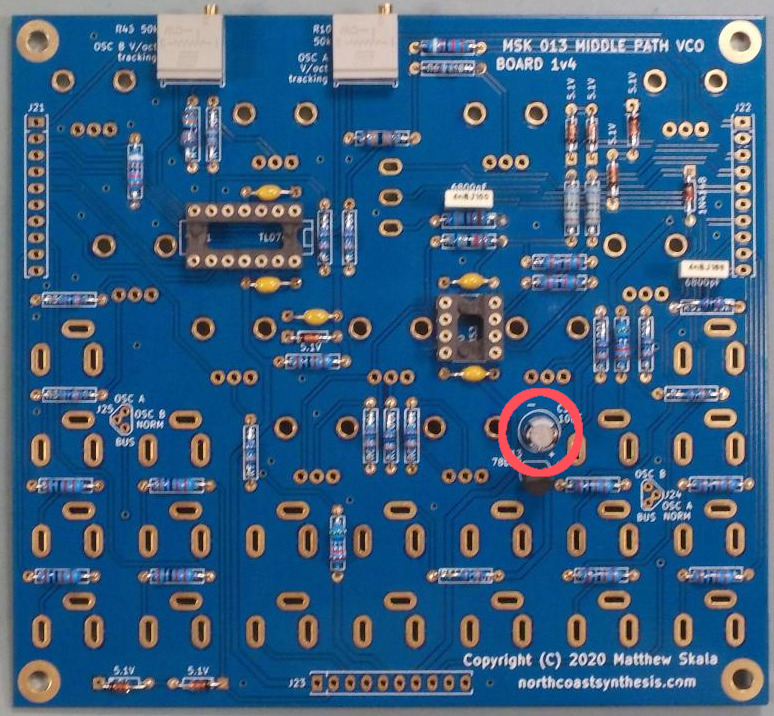
\includegraphics[width=\linewidth]{cap-10u1.jpg}

\section{Board to board connectors}

Fasten the four 10mm standoffs on the back of Board~1; that is the side
opposite the components already installed.  The male ends of the 10mm
standoffs should pass through the mounting holes in the board and mate with
the female ends of the 11mm standoffs on the front or component side of the
board.  Be careful to get right which standoffs are the shorter ones (10mm)
and which are the longer ones (11mm).

Mate the three pairs of 10$\times$1 header connectors J21--J23 and P2--P4
and place them (do not solder yet) in the J21--J23 footprints on Board~1
with the legs of the female connectors going through the board.

\nopagebreak
\noindent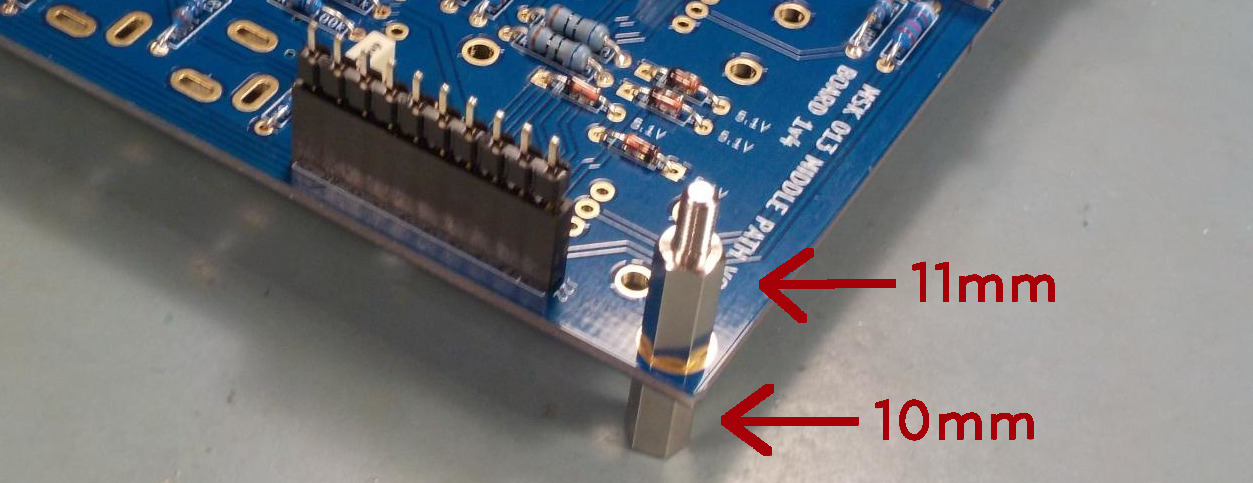
\includegraphics[width=\linewidth]{standoffs.jpg}

Place your completed Board~2 from the previous chapter on top of the
assembly, component side up with the legs of P2--P4 going through the
footprints on the back of the board, and fasten the board to the 11mm
standoffs with the four hex nuts.  The resulting temporary assembly should
be as shown in the photo.

\nopagebreak
\noindent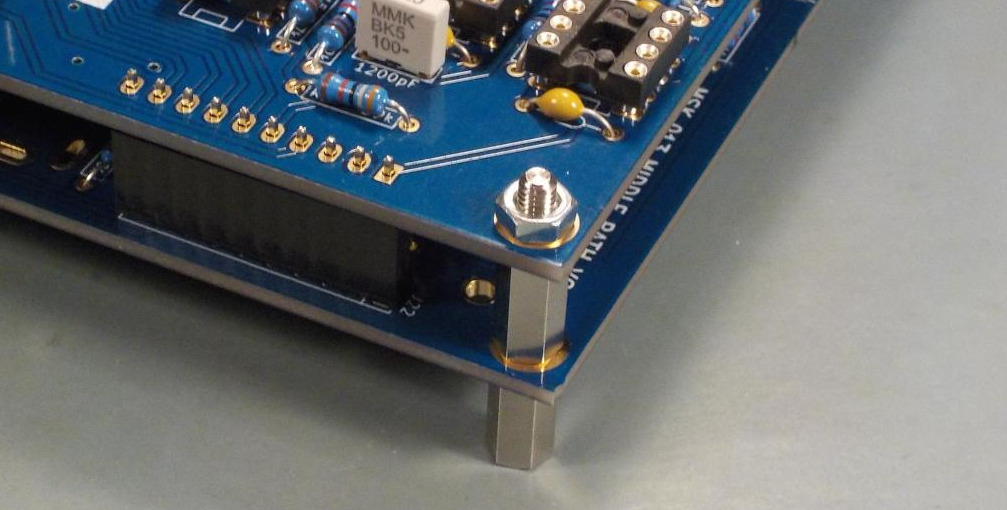
\includegraphics[width=\linewidth]{temp-assy.jpg}

Solder J21--J23 and P2--P4 in place on the two boards.  Then remove Board~2
and the hex nuts holding it in place, but keep the standoffs attached to
Board~1.

\section{Panel components}

Flip Board~1 over; you will now be installing the components that go between
it and the panel.  The pieces fit together in a straightforward way, but
see the exploded assembly diagram on page~\pageref{fig:exploded} if
further clarification is needed.

Remove any hardware such as nuts and washers that may be supplied
pre-threaded onto the panel components and set all that stuff aside before
proceeding.

Place (do not solder yet) the twenty phone jack sockets J1--J20 in
their footprints.  These are for patching signals to and from other modules. 
These components should only be able to fit into the board in one way.

\nopagebreak
\noindent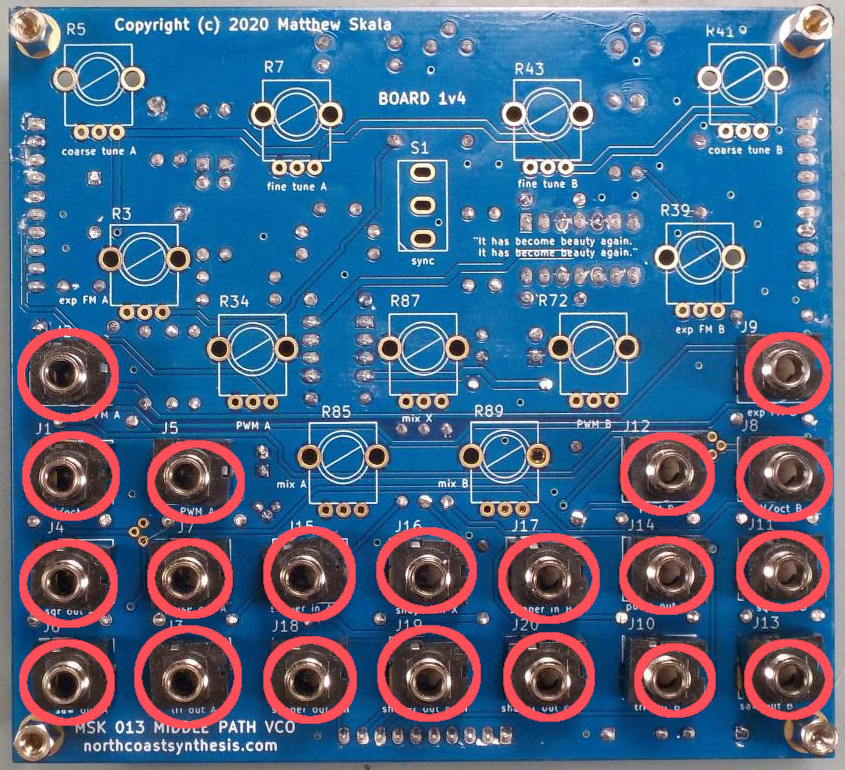
\includegraphics[width=\linewidth]{jack-sockets.jpg}

Place (do not solder yet) the eleven panel control potentiometers R3, R5,
R7, R34, R39, R41, R43, R72, R85, R87, and R89 in their footprints.  These
components, too, should only be able to fit into the board in one way.

\nopagebreak
\noindent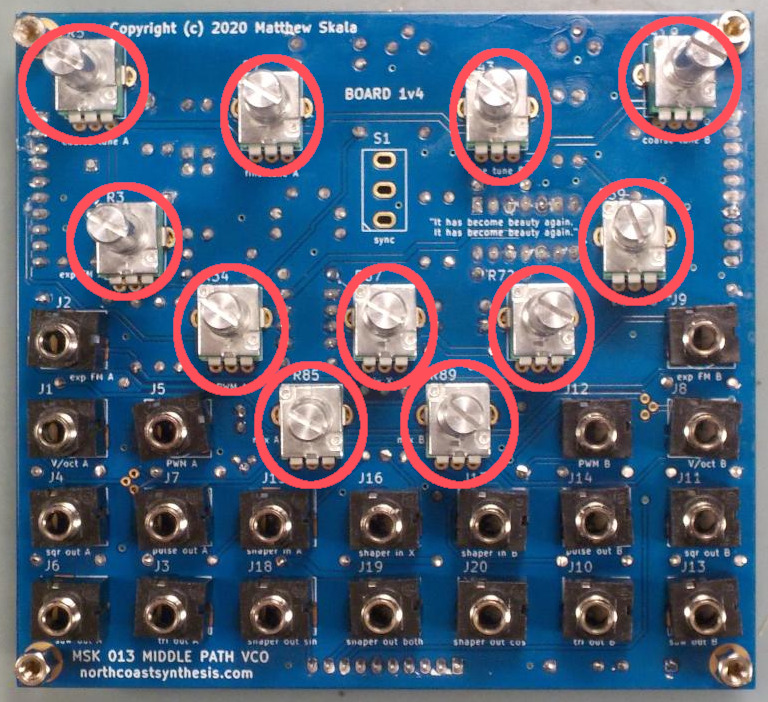
\includegraphics[width=\linewidth]{panel-pots.jpg}

Place (do not solder yet) the toggle switch S1 in its footprint.  This
switch is used to select the sync mode.  The electrical connections on this
switch are symmetrical, but there is a keyway or groove on the threaded
bushing of the switch, and the keyway must be oriented downward for the
mounting hardware to fit properly later.

\nopagebreak
\noindent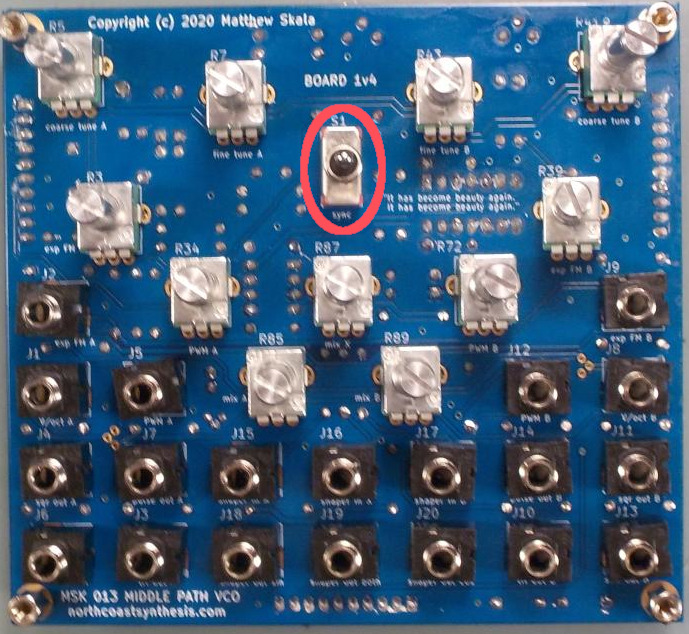
\includegraphics[width=\linewidth]{spdt.jpg}

Line up the panel on top of the assembly.  Fasten it in place by driving
the four machine screws through their corresponding holes into the 10mm
standoffs.

Install all the hardware for the panel components.  The potentiometers will
each have one washer and one hex nut; the washer goes on first,
nearest the panel.  In the case of the jack sockets, the knurled nuts
provided for these will have screwdriver slots on one side, and those should
face the outside with the smoother side facing the panel.  The switch should
have a locking ring with a little tooth that fits into a hole just below the
bushing; this will only work properly if you put the switch into the board
in the correct orientation.  The locking ring goes closest to the panel,
followed by a toothed lockwasher and two nuts.  The sharper points on the
lockwasher should point out, facing the nut, if one side feels sharper than
the other.

Do not overtighten any of this hardware, and be careful, if you are
using wrenches or pliers, to avoid scratching the panel.  Wrapping the tool
jaws with tape may help.

\begin{figure*}[b!]
\noindent\hspace*{\fill}%
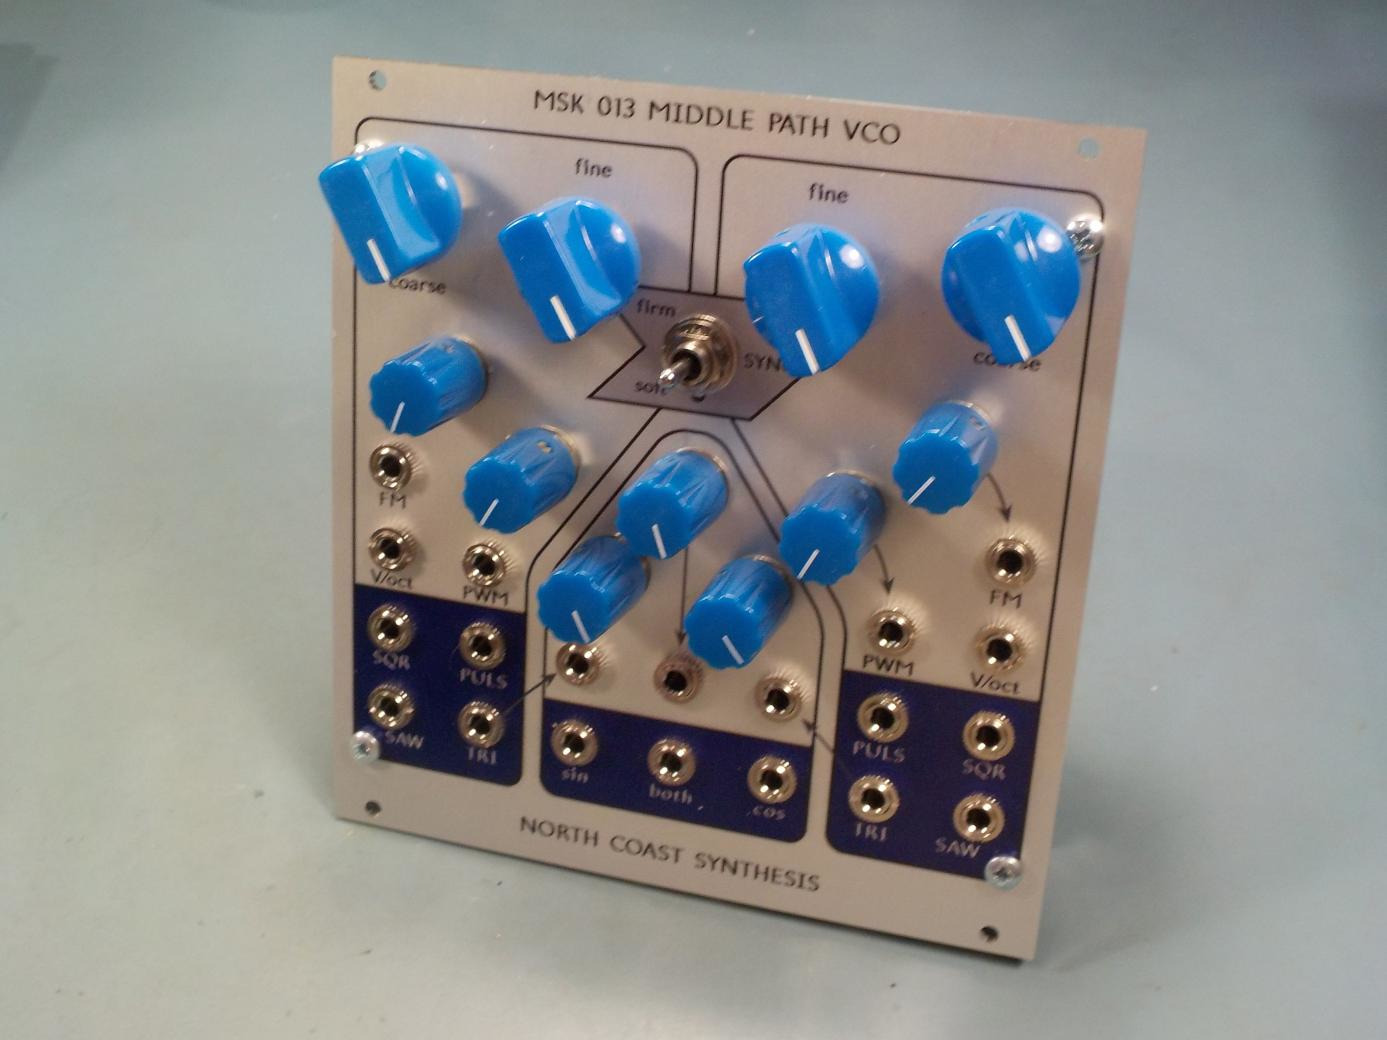
\includegraphics[width=4.4in]{module-complete.jpg}%
\hspace*{\fill}\par
\end{figure*}
\addtocounter{figure}{-1}

\section{Final assembly}

Insert the LF353 chip U10 in its socket on Board~1.  Be careful to insert it
right way round:  the end with Pin 1 will be marked by an
indentation at one corner or a notch in the end and this end of the chip
should be inserted to match the notch in the socket and on the board
silkscreen and the rectangular Pin 1 solder pad.  The Pin 1 end of the chip
is at the bottom when the module is inserted in a rack.

Also be careful that all the legs of the chip go into the corresponding
holes in the socket.  These chips, when brand new, usually have their legs
splayed outward a little bit (a measure intended to help them fit snugly
into circuit boards when used without a socket) and you must gently bend the
legs inward in order to fit them in the sockets.  If you apply
pressure to a chip prematurely, without all the legs properly fitting into
the holes, it is easy to have the legs fold up or even break off.

Similarly, insert the TL074 chip U1 in its socket on Board~1.  The same
general comments on installing DIP chips apply here.

It should not be necessary to remove the panel from Board~1 again.  Just
attach Board~2, carefully fitting its header plugs into the header sockets
on Board~1 and the male ends of the standoffs through the corresponding
holes in Board~2.  Then use the hex nuts to fasten Board~2 in place.

Insert the LF353, TL074, LM13700, THAT320, and AD633 chips in their sockets
on Board~2.  Be careful to insert them right way round, with the Pin~1
markings on the chips matching those on the board.  As with the chips on
Board~1, be careful all the legs are in the holes of the socket before you
press each chip down, lest you fold up the delicate legs.  Also be careful
not to confuse which chip goes in which socket; and be especially careful
with the THAT320 and AD633 chips.  They are expensive.

\pagebreak

Add the knobs.  Be careful not to overtighten the setscrews; they have a
tendency to strip.

There is a rectangular white area on Board~2, just above the sine shaper,
reserved for adding a serial number, signature, quality control marking, or
similar.  Use a fine-tipped permanent marker to write whatever you want
there.  Isopropyl alcohol will probably dissolve marker ink, so do this step
after any board-cleaning.

\nopagebreak
\noindent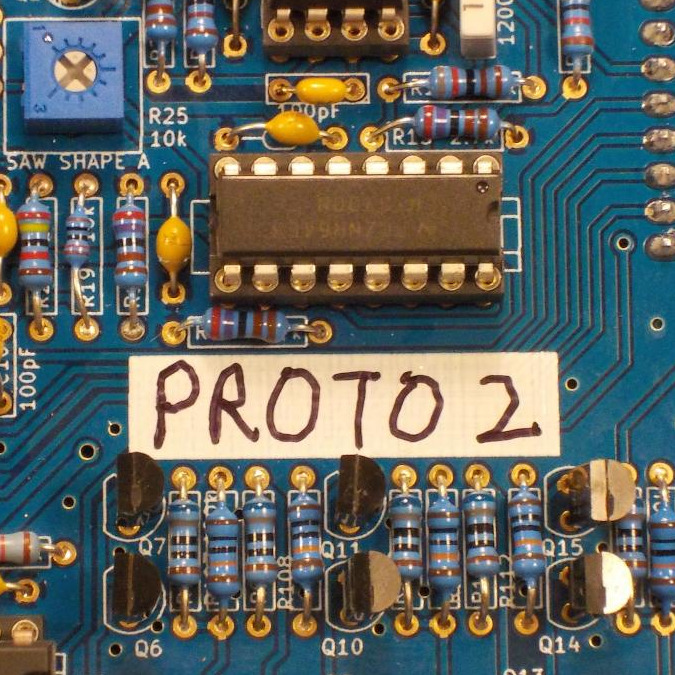
\includegraphics[width=\linewidth]{serial.jpg}

Your module is complete.
